% Created 2017-04-07 Fri 16:17
% Intended LaTeX compiler: pdflatex
\documentclass[sigconf]{acmart}
\usepackage[utf8]{inputenc}
\usepackage[T1]{fontenc}
\usepackage{graphicx}
\usepackage{grffile}
\usepackage{longtable}
\usepackage{wrapfig}
\usepackage{rotating}
\usepackage[normalem]{ulem}
\usepackage{amsmath}
\usepackage{textcomp}
\usepackage{amssymb}
\usepackage{capt-of}
\usepackage{hyperref}
\author{Nick Merrill, Max Curran, John Chuang}
\affiliation{%
  \institution{BioSENSE, UC Berkeley School of Information}
  \city{Berkeley} 
  \state{California, USA} 
}
\email{ffff@berkeley.edu}

\hypersetup{
 pdfauthor={},
 pdftitle={},
 pdfkeywords={},
 pdfsubject={},
 pdfcreator={Emacs 25.1.1 (Org mode 9.0.4)}, 
 pdflang={English}}

\begin{abstract}
While brain-computer interfaces are used by some individuals with disabilities,
passthought authentication stands a chance at becoming the first brain-computer interface to reach wide, consumer adoption.
However, to move passthoughts out of the lab and into the world, 
we will need both quantitative data about EEG signals 
and rich, qualitative data about user beliefs surrounding EEG specifically, and the possibility of mind-reading devices generally.
\end{abstract}

\keywords{passthoughts, authentication, usable security}


\setcopyright{rightsretained}
\acmDOI{10.475/123_4}
\acmISBN{123-4567-24-567/08/06}
\acmConference[NSPW '17]{New Security Paradigms Workshop}{October 2017}{Islamorada, Florida, USA}
\acmYear{2017}
\copyrightyear{2017}
\acmPrice{15.00}
\date{\today}
\title{Is the Future of Authenticity In Our Heads?\\\medskip
\large Moving Passthoughts From the Lab to the World}
\hypersetup{
 pdfauthor={},
 pdftitle={Is the Future of Authenticity In Our Heads?},
 pdfkeywords={},
 pdfsubject={},
 pdfcreator={Emacs 25.1.1 (Org mode 9.0.4)}, 
 pdflang={English}}
\begin{document}

\maketitle

\section{Introduction}
\label{sec:org87242b0}

Usable authentication is a long-standing problem in computer security.
Traditional passwords are easy to guess and difficult to remember,
while biometric authenticators like fingerprints are easy to steal and difficult to change.
Possession of tokens or keys are susceptible to loss, 
and the use of multiple factors (such as password and SMS) require multiple steps, hindering wider adoption.

First proposed by \cite{Thorpe2005}, ``passthoughts'' authentication allow users to 
to submit both a knowledge factor (i.e., secret thought) and an inherence factor (i.e., brainwave signal unique to the individual) 
in a single step, by thinking a single mental task.
Even better, passthoughts have no externally visible ``tell,'' making them impervious to shoulder surfing attacks.
Passthoughts has been validated in a controlled environment using consumer-grade EEG devices with a single electrode \cite{Chuang2013b}, 
and using earpieces that collect EEG from the ear \cite{curranpassthoughts}.
\cite{Johnson2014} showed this protocol to be robust against impersonation attacks, even when the attack has learned the target's secret thought.
While recent work is heartening, passthoughts remains confined, for now, to the lab.
This paper reviews the immediate questions that must be addressed if passthoughts is to move into everyday life.

First, we must test passthoughts in a variety of conditions: ambulatory settings, under different levels of stress, drowsiness, caffeine or alcohol, etc.
Through this work, we may build a better understanding of the statistical distribution of EEG signals that a person gives off during the course of their life. 
This statistical analysis will help us understand the space of possibile passthoughts. 
It will also help us estimate how easy or difficult passthoughts are to guess, or crack.

Second, we must understand the real usability properties of passthoughts.
While much work has claimed passthoughst to be more usable than traditional multi-factor authentication protocols,
as of yet, no work systematically evaluates this claim.
The usability of passthoughts authentication will depend not only on its performance in ecologically valid contexts,
but also on people's attitudes about brainwaves, EEG, and biosensing generally.
Past work indicates that people believe EEG can reveal what someone is thinking or feeling, which could scare off wider adoption (Section 4).

The main goal of this paper is to motivate and contextualize immediate studies that can address the above issues.
Section 5 proposes two, complementary studies.
The first proposed study focuses on the use of passthoughts in a realistic, though lab-constrained setting.
By fixing some parameters (context of use, and feedback to the user), this study would allow a first look at how passthoughts might work
in a real-time application context.
The second proposed study focuses on people's longitudinal relationships with EEG in their everyday life.
This study focuses not on differences in behavior between experimental conditions, but on evolving attitudes (and changing signals) over time,
as a way of assessing both dynamic user attitudes, and the possible impact of shifting neural signals.

Passthought authentication stands a chance at becoming the first brain-computer interface to reach wider adoption. 
As such, passthoughts promises not only more usable, multi-factor authentication,
but also a source of data for those attempting to build other brain-computer interfaces,
The strategy is not without risks (Section 6),
but, if future work can address the two challenges posed here, several interesting paths unfurl.
e.g. for people with motor disabilities \cite{Mattia2013}.
closed-loop authentication, continuous and/or tacit authentication, 
and possible theoretical contributions to neuroscience, authentication and HCI (Section 7).

\label{fig:earbud}
\begin{figure}[htbp]
\centering
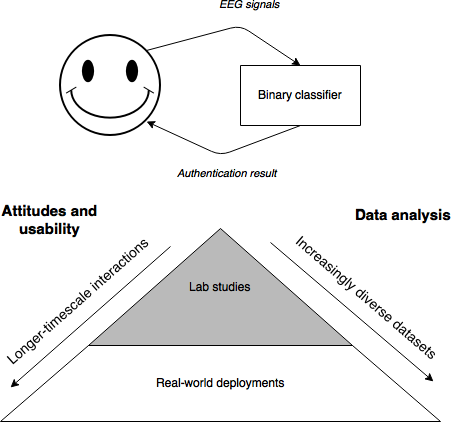
\includegraphics[width=.9\linewidth]{./figures/passthoughts-diagram.png}
\caption{A passthought authenticator.}
\end{figure}

\section{Background}
\label{sec:org1286678}

Authentication is the act of proving that a user is who they claim to be.
In computer security, authenticators are classified into three types: knowledge factors (e.g., passwords
and PINs), possession factors (e.g., physical tokens, ATM cards), and inherence
factors (e.g., fingerprints and other biometrics). 

An ongoing problem in authentication lies in balancing strong security
(i.e., combining multiple factors of authentication)
with usability.
As an example, major industry players such as Google and
Facebook have strongly encouraged their users to adopt two-factor
authentication (2FA), in which a user enters his or her password (a knowledge factor),
and subsequently receives a code on their cellphone (a posession factor).
However, submitting two different 
authenticators in two separate steps has frustrated wide adoption
due to its additional hassle to users. The Apple iPhone, for instance,
already supports device unlock using either a user-selected passcode or a fingerprint. The
device could very well support a two-step two-factor authentication scheme if
desired. However, it is easy to understand why users would balk at having to
enter a passcode \emph{and} provide a fingerprint each time they want to unlock their phone.

\subsection{One-step, multi-factor authentication}
\label{sec:orgc34f372}

To assist with the usability issues surrounding multi-factor authentication,
passthoughts aims to provide two factors of authentication in a single step.
A single mental task, or passthought, provides both a knowledge factor (a chosen secret thought)
with an inherence factor (the way that thought is expressed for an individual) \cite{Chuang2013b,Johnson2014}.
Using a custom sensing device, passthoughts could provide an additional posession factor, all in the same step.

Other work has attempted to provide multiple factors of authentication in one step.
Some work has tested behavioral authentication methods such as keystroke dynamics, or voice. In both cases, the knowledge factor (password or passphrase) and
inherence factor (typing rhythm or speaker's voice) are employed \cite{Monrose1997}.
In contrast, the Nymi band supports one-step two-factor authentication via the inherence
factor (cardiac rhythm that is supposed to be unique to each individual) and the
possession factor (the wearing of the band on the wrist) \cite{Nymi}.
Custom-built EEG devices could incorporate an added possession factor 
to the already two-step authentication provided by passthoughts \cite{Curran2017}.

Authenticators are susceptible to a variety of attacks. 
One common attack on passwords is ``shoulder surfing,'' in which an attack uses visual or other cuesto steal, or improve the chances of guessing, a target's chosen secret. 
Passthoughts mitigates this attack by nature of the mental gesture:
since the expression of a passthought is not externally visible, the authenticator is impervious to shoulder surfing attacks.

\subsection{Passthought authentication}
\label{sec:orga70a9dc}

The use of EEG as a biometric signal for user authentication has a short history.
In 2005, Thorpe et al. motivated and outlined the design of a passthoughts system \cite{Thorpe2005}. Since 2002, a number of independent groups have achieved low (less than 1\%) false acceptance rates using multi-channel sensors placed on the scalp \cite{Poulos2002,Marcel2007a,Palaniappan2008,Ashby2011}.
In 2013, one group showed that similar accuracy can also be
achieved using a consumer-grade single-channel sensor \cite{Chuang2013b}. 
In particular, the lack of signal diversity from multiple EEG channels can be overcome by allowing
the users to choose their own personalized passthoughts (e.g., sing their favorite
song in their head). There are two significant consequences of this result. First,
the passthoughts approach is no longer constrained by the high cost (> \$10,000 USD)
and low usability (gel-based electrodes; aesthetic challenges of an EEG cap) of
medical-grade multi-channel devices. Second, because users can choose and
easily change their secret mental task, this approach can support one-step two-
factor authentication via the simultaneous presentation of the inherence factor
(brainwave signatures due to the unique folding structures of the cortex) and the
knowledge factor (the secret mental task) \cite{Chuang2014}.

\subsection{Passthoughts using in-ear EEG}
\label{sec:orge2da838}

Even consumer-grade headsets can be uncomfortable to wear, and are awkwardly visible to outside observers. Earbuds present a more discreet, comfortable location for an EEG sensor, as many people already wear earbuds in day-to-day life.

\label{fig:earbud}
\begin{figure}[t!]
\centering
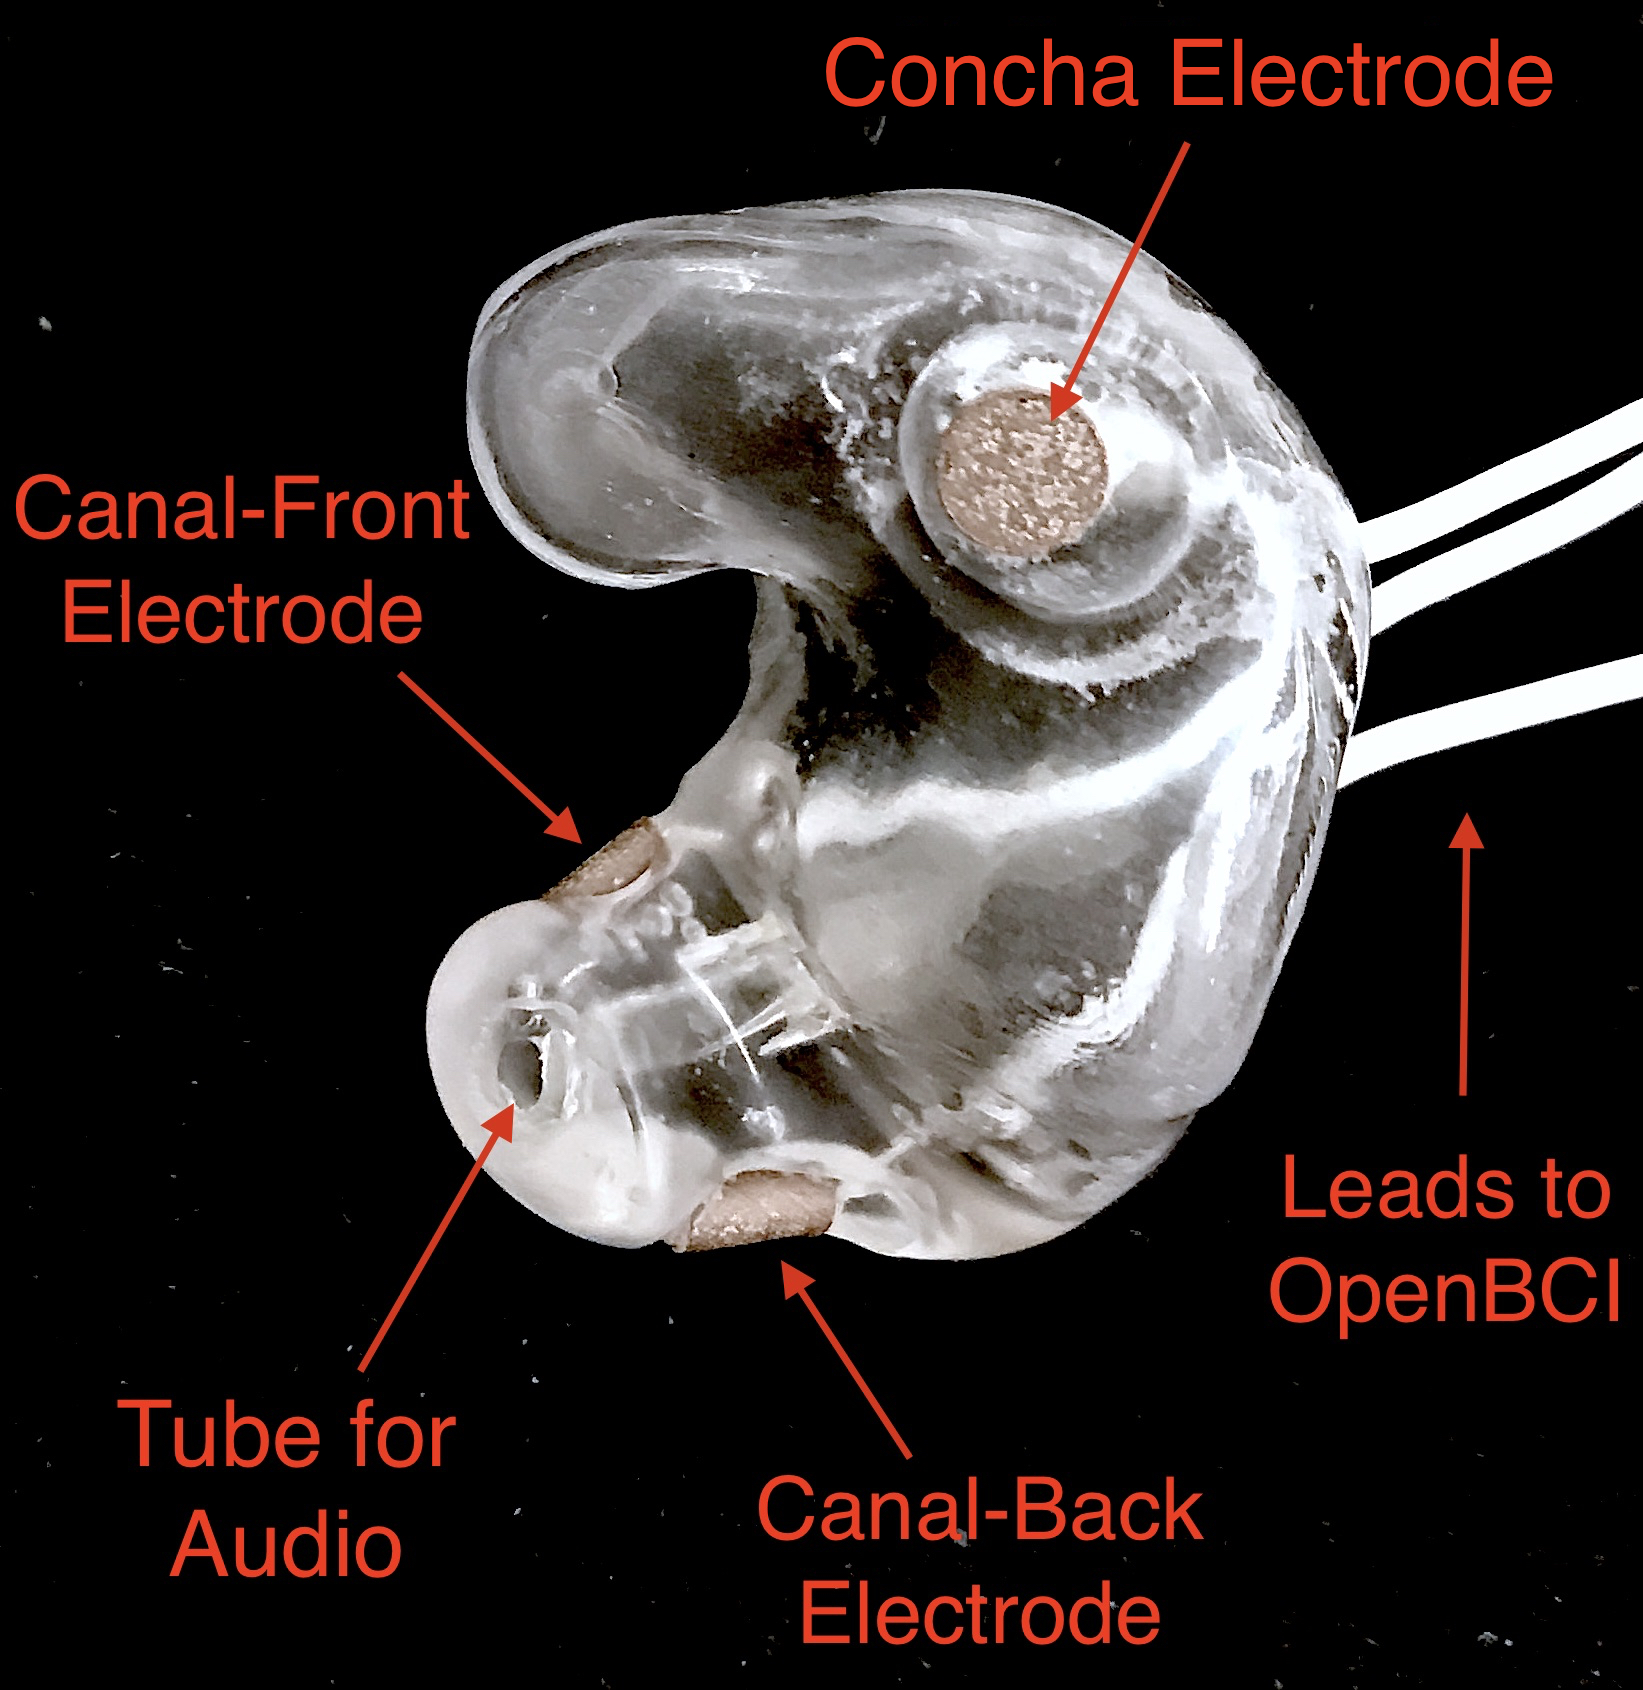
\includegraphics[width=.9\linewidth]{./figures/custom-fit-eeg-annotated.jpg}
\caption{A custom-fit in-ear EEG device as used in Curran et al, 2017}
\end{figure}

Research in in-ear EEG is only several years old. Nonetheless, the concept has
attracted a lot of attention because of the discreetness factor of in-ear EEG over
traditional scalp-based EEG. A research team at the Imperial College London
and Aarhus University published a landmark paper in 2011 that introduced the
concept of in-ear EEG, demonstrating for the first time the feasibility of recording
brainwave signals from within the ear canal
\cite{Looney2011}.
Follow-up work from the same
group demonstrated its ability to produce signal-to-noise ratios comparable to
those from conventional EEG electrode placements, robustness to common
sources of artifacts, and use in a brain-computer interface (BCI) system based on
auditory evoked potentials and visual evoked potentials
\cite{Looney2012a,Kidmose2013a,Kidmose2013b}.


\cite{curranpassthoughts} was the first to merge in-ear EEG with passthought authentication,
 using a modified consumer grade EEG device with a single electrode, achieving approximately 80 percent authentication accuracy. 
Ongoing work from the same authors investigates the use of custom-fit earbuds with multiple embedded electrodes \ref{fig:earbud}.
Lending credibility to that study's claim that in-ear EEG could one day become feasible in consumer devices,
United Sciences recently announced a consumer "hearable'' (in-ear wearable) called The Aware, which will measure EEG from the ear, among other biometrics \cite{UnitedSciences}.

\subsection{Contending with mind-reading machines}
\label{sec:org463ed13}

Finally, a crucial thread of past work work concerns how users perceive the capabilites of devices that purport to ``read'' their ``mind.''
Biosensing devices in general raise many questions for consumers.
You might be eligible for an insurance discount if you wear a FitBit \cite{Bernard2015} (depending, of course, on what readings the FitBit produces \cite{Brain2015}). 
But, would you wear a device in the workplace \cite{solon2015}, if your manager used it to track your productivity?
If biosensor data can be used in the courtroom \cite{Crawford2014}, could not pervasive biosensing help to \emph{predict} crime \cite{Thompson2011}? 
After all, one study suggests that probability of involvement in violent crime can be predicted from one's resting heartrate \cite{Latvala2015}. 

In all of these examples, biosensing technologies blur the line between \emph{sensing bodies} and \emph{sensing minds}. 
Now, when people decide to buy sensor-equipped consumer devices \cite{Stables2016}, or get sensed passively by devices integrated into the walls and ceilings \cite{Adib2015} or city streets \cite{Thrift2014}, end-users will need to contend with the prospect of mind-reading machines.

If people \emph{think} a certain technology measures aspects of mind, it will certainly affect the way they engage with that technology - whether or not it works the way they expect \cite{Ali2014a}. Meanwhile, if they think that a given technology does \emph{not} measure their mind, when it fact it does, users may suffer a breach of what Nissenbaum might call the ``appropriateness of the flow of information'' \cite{Doyle2011}. In both cases, knowing what people expect will help us anticipate their needs, and concerns.

Crucially, there are some people who actually \emph{want} their minds measured, e.g. for self-reflection. Consider the Spire, a breath sensor that claims to divine, from a person's patterns of in-breaths and out-breaths, what the user is calm, focused, or tense \cite{SpireInc}. 
For the device to ``work,'' not only must these detected signals match with end-users' intuitions, but users must also believe that a device like the Spire has the power to measure and detect these phenomena, given breath as input \cite{Ali2014a}. 
In general, technologies that claim to ``measure the mind'' must rely on end-users to define the criteria by which systems are deemed effective, or accurate. 

If we wish to understand what role passthought authentication \emph{could} play in day-to-day life,
we must view it both through the lens of potential privacy concerns, \emph{and} through the lens of possible opportunities for self-reflection and self-understanding. 
Of course, users' attitudes will not be fixed: they will evolve over time, as users observe the device in action, and correlate its judgments with their own lived experiences \cite{Nafus2016}.

\section{Diversity and crackability of passthoughts}
\label{sec:org8b8d857}

To transition from the lab to the real world,
passthoughts studies must collect larger, and more diverse corpora of EEG data.
While past work on passthoughts has achieved excellent results on corpora of recordings from different users, 
these studies do not consider passthoughts from a variety of different subject conditions.
For example, sitting subjects may have different patterns of neural activity from subjects who are standing, walking or exercising \cite{Thibault2016a},
let alone subjects who are under the influence of caffeine, alcohol or marijuana.

Relatedly, these studies do not systematically investigate how these recordings relate statistically to non-passthoughts.
That is, we do not know how the particular passthoughts observed in past work are drawn from the distribution of EEG signals that an individual produces over the course of their day.
This blind-spot poses a possible challenge to passthought's vulnerability to dictionary-style cracking.
If I have a large enough corpus of EEG readings, do some passthoughts start to look as guessable as \emph{password1234}?
By answering such questions, we could design data-driven policies for, e.g., how many retry attempts passthought authenticators should allow.
Investigating this question could also help us understand how and why passthoughts work at all: Why are passthoughts unique, and how unique are they?

\section{User Perceptions of EEG}
\label{sec:orgd436f39}

The prior section outlined the first major challenge to passthought authentication: that of corpus diversity.
The following section reviews a more subtle challenge: that of usability, as it relates to attitudes around sensing brainwaves.

What can machines know about a person's mind, even theoretically? 
This question is never more relevant than when speaking of attempts at quantitative measures of brain activity (e.g. brainwaves).
Past work has established the almost magical abilities that people tend to ascribe to brain-scanning devices, even subjects with specific training in the limitations of brain-scanners \cite{Ali2014a}.
This section outlines concerns around ``mind-reading'' machines, and how they relate to EEG and passthoughts specifically.
We then move to a discussion for possible ways to address these concerns, and concerns about dataset diversity, in the following section.

\subsection{What (do you think) EEG can reveal about a person?}
\label{sec:orgad4f714}

In our preliminary findings, brainwaves (EEG) are seen as among the most revealing biosignals, just below body language and facial expression, in their capacity to reveal the goings on of a person's mind. 
More common sensors such as GPS and step count are seen as less revealing (despite empirical evidence suggesting such data can be quite revealing indeed \cite{Canzian2015}).

The survey I report on here, currently in-progress, examines how people's beliefs differ given device ownership, and their membership in one of two groups: Mechanical Turk workers, or people enrolled in Health-e-Heart, a massive (n > 40,000), longitudinal study, in which volunteers fill out surveys about themselves, and/or upload data from biomedical self-tracking devices, over the course of several years \cite{Estrin2010a}.
In one portion of the survey, we ask subjects to rate a number of different biosensors in order of how likely individual's believe each sensor is to reveal what ``a person is thinking or feeling'' (Figure \ref{fig:rank}).

\label{fig:rank}
\begin{figure*}
\centering
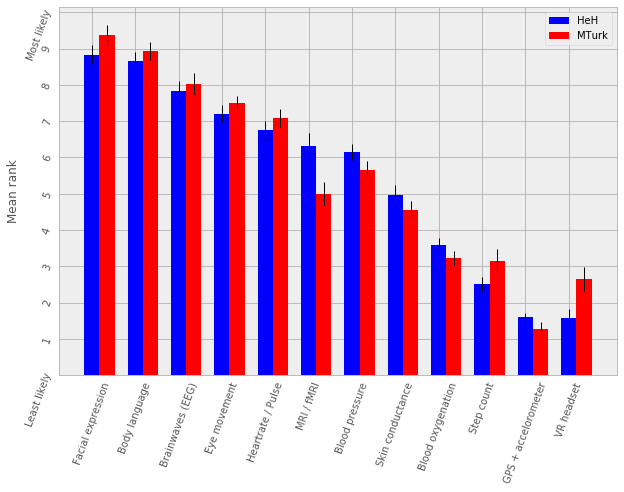
\includegraphics[width=.9\linewidth]{./figures/rankings.png}
\caption{``Please rank the following sensors in how likely you believe they are to reveal what a person is thinking and feeling.'' Mean Likert responses (Not at all\ldots{}Very informative). Lower bars mean higher rank (1 being the highest-ranked,  or most likely to reveal what one is thinking or feeling.''}
\end{figure*}

What will this finding mean for wider adoption? 
Will people shy away from using their passthought authenticator in certain situations, or when they are feeling some type of way?
The following section describes one exploratory study that could investigate some aspects of this larger question.

\section{Two studies on passthoughts}
\label{sec:org0426e70}

This section proposes two studies on passthought authentication.

\subsection{A real-time passthought authenticator}
\label{sec:org85dc730}

Past work has proposed passthoughts as a more usable form of multi-factor authentication,
as compared to existing protocols.
However, no study yet has systematically evaluated this claim.
Here, we propose a study aimed at 
examining passthought's usability in an ecologically valid context.

This study would take place in a lab, under the supervision of an experimenter.
First, the experimenter would calibrate a subject with a passthought authenticator, as in \cite{Chuang2013b}.
Through an automated cross-validation process, the participant's best-performing passthought would be selected.

Next, the experimenter sould present users with an online banking application, and ask them to perform their passthoughts.
We can manipulate feedback such that users either see the real authentication accuracy (control), 
are always rejected by the authenticator, 
or always accepted by the authenticator.

\subsubsection{The effect of feedback}
\label{sec:org63fcbe5}

Through this study, we might find 
that passthoughts is considered usable, even when authentication attempts are always rejected.
We might also find that passthoughts are not considered usable, 
even when authentication attempts are always accepted.

Furthermore, using the data collected during this study, we could perform an offline analysis 
to test for the effect of these conditions on the actual performance of users' passthoughts, and consequential classifier accuracy.
When subjects are continuously rejected, do their passthoughts change in frustration (or in an attempt to gain access)?
We might find that passthought performance 
remains stable, regardless of what feedback subjects are shown.
Alternatively, we might find that performance changes 
when subjects are continuously rejected from their authenticator.
Alternatively, performance may change, 
even when subjects are continually accepted by their classifier.

This study's findings could have far-reaching impacts for the future development of passthought authenticators.
Its results would shed light on how passthoughts change as a response to authenticator performance on one hand,
and how authenticator performance affects perceptions of passthoughts' usability on the other.

\subsubsection{Exploring continuous re-calibration}
\label{sec:orgc3c28b6}

In addition to these findings, the data generated during this study could help test 
a third hypothesis: that the continual re-training of passthought classifiers might help boost classification performance over time,
especially in the face of shifting signals.
Offline, we can train each classifier, for each subject, to achieve its post-calibration state.
Next, we can run each reading recorded from a particular participant through the trained classifier.
If the classifier accepts the reading, we can then re-train the classifier, 
adding this reading to the corpus of positive examples.
In a separate, \emph{negative calibration} condition, 
we also re-train the classifier with rejected readings as negative examples.

By comparing the final FAR and FRR for each subject using these strategies, 
compared to the one-time calibration strategy, we could begin to get an idea as to whether
this strategy helps achieve superior performance, especially when signals change.
This analysis could also act as a harbinger for some of the possible downsides of this approach:
If a user is continually rejected, and the classifier is re-trained using those rejections as negative examples,

\subsection{A longitudinal study on brainwave monitoring}
\label{sec:orgd647693}

The study proposed above would help answer preliminary questions about
the usability of a passthought authenticator,
and possible ways for dealing with shifting neural signals.
However, as reviewed above, two major challenges would still remain for passthoughts authentication.

First, we do not have a sufficiently large corpus of EEG signals, 
preventing us from investigating how robust passthoughts authentication performs in various user conditions,
and from understanding how easy particular passthoughts are to guess or crack.
Second, we do not understand how people's beliefs about EEG might affect their behavior with a passthought authentication system.
Unfortunately, these challenges make it difficult to produce a passthought authenticator that works with any reliability in real contexts,
making, a longitudinal study with a working authenticator not immediately practical.

However, we may still perform a longitudinal study that allows us to interrogate the usability aspects around (and attitudes about) passthoughts specifically, and EEG generally.
In so doing, we may also collect a larger and more diverse corpus of passthoughts, which can be used to address the paucity of data we face today.
A technology probe or diary study \cite{Gaver1999} could help address both of these issues at the same time 

A small group of subjects could wear a working, recording EEG device, whether or not it provides feedback, in a variety of settings for some number of days,
having subjects journal their experiences and asking them specifically what they feel someone might be able to know about them from the EEG signals they record.
At the same time, we could use this study as an opportunity to collect a much larger, and more diverse corpus.
To aid in the collection of signals that are specific to our problem of passthought authentication,
subjects in this study might be prompted to perform a variety of tasks at a few pre-chosen points throughout the day.
With the data collected during this study, we could easily simulate passthought accuracy on a much more realistic (and representative) sample of readings.

Such a study would trade a large population size for a large corpus of diverse data.
This tradeoff allows us to closely investigate the diversity of EEG signals within subjects.
The diverse readings encountered in day-to-day life could help us understand how such signals change as a function of time, and/or in different psychophysical states.
At the same time, our small sample size could enable a rich, qualitative understanding of users attitudes.

The following two sections expand on both aspects of this project in greater detail.

\subsubsection{A more diverse corpus}
\label{sec:org6aad8bd}

While subjects wear their EEG device and diary about their experience, we should also ask subjects to perform
targeted mental tasks (potential passthoughts) in a variety of contexts (ambulatory, under the influence of caffeine or alcohol, etc). 
This diverse corpus should allow us to both evaluate performance in ambulatory settings, and to
investigate the possibility that past works' models overfit for subjects who are sitting down in a lab.
How do an individual's EEG signals change throughout various activities, and mental states?

This corpus will, of course, also include unlabeled non-task data from similarly diverse settings, perhaps concurrent with streams of GPS or accelorometer data.
Unlabeled data represents another fruitful source of data for passthoughts.
The unlabeled samples in this corpus also allow us to examine properties of EEG signals in general, helping us build more robust models which should help us prevent overfitting in the future.

In another potentially fruitful analysis, such a corpus will allow us to perform statistical analysis of how passthoughts are drawn from the overall distribution of EEG signals. 
Using multi-dimensional clustering algorithms such as tSNE \cite{VanDerMaaten2008} 
could assist us in understanding how particular passthoughts relate to other EEG signals that an individual expresses involuntarily throughout the day. 
These clusters will help us understand how rare or unlikely a given passthought is, and help shed light on why and how given passthoughts are expressed uniquely between individuals.

Leveraging the statistical clusters of EEG data generated by these algorithms, it might also be possible to generate a ``passthoughts cracker,'' capable of generating plausible passthoughts. 
Feeding these algorithms into pre-trained passthought classifiers, we can begin to generate realistic models of classifiers' resistance to cracking attempts. 
These cracking experiments could lead to defenses against cracking attempts, by enforcing retry attempt timeouts or other methods for limiting break-in risk, such that strong guarantees can be enforced.

\subsubsection{Usability and attitudes}
\label{sec:orgd8e2296}

By deploying a real sensing apparatus, be it a traditional consumer device such as the Muse \cite{Mihajlovic2015} 
or a more experimental piece of equipment such as an earbud \cite{UnitedSciences}, 
and having people record EEG data in their daily life, we could learn more about the interpretative qualities of these data  \cite{NafusDawn;Sherman2014}.
Such a study presents a dual opportunity to understand user beliefs in a rich, qualitative sense, while simultaneously collecting the large, diverse and longitudinal corpus of EEG signals necessary if we wish to stand a chance at decent classification accuracy in the wild.

Of course, this study is no substitute for a working, online passthoughts authentication system.
Instead, this study aims to collect useful data before such a system exists.
It will not only elicit beliefs, 
but also allow us to collect larger datasets, 
and to catch technical issues in sensing devices and collection platforms.

\section{Privacy, Security: Choices, Tradeoffs}
\label{sec:orgd1ac1ca}

After the study described above, future work should be able to start building more robust, world-ready passthought systems,
which could offer improvements to the usability and security of authenticating.
However, these opportunities do not come without risks. 
Indeed, some risks are unique to the application context, and to EEG as a class of biosignal. 
This section briefly reviews risks to user privacy and security that widespread passthought authentication may introduce. 
I do not pose specific challenges to passthoughts here, though many surely lurk; instead, I present broad class of categories from which questions may emerge. 

\subsection{Privacy}
\label{sec:org3b2cea6}
One clear risk comes to user privacy, as it is still not well understood what EEG signals might reveal about a person.
EEG signals that are not anonymized could, at least theoretically, come to be seen as private in the face of new methods of analysis.
(If your brainwaves can authenticate you, could they also uniquely identify you, even if your name is redacted?)
Differential privacy \cite{Dwork2014} presents one approach to dealing with the risk of privacy breaches with EEG signals.
By adding noise to datasets, differentially private databases can make strong guarantees about the likelihood of a de-anonymization attack on particular datbase queries.

\subsection{Security}
\label{sec:org7d15f96}
Device security presents another risk to passthought authentication.
Since EEG devices will transmit data, likely wirelessly \cite{Mihajlovic2015}, their data may be intercepted, depending on the security properties of the underlying transit protocol. 
When transferring authentication credentials in passthoughts, the ability to snoop on authentication attempts could present a dangerous attack vector.

There is also the question of the security of large data repositories in which EEG data might be stored.
Large data repositories are what Wolf \cite{Wolf2010} calls a ``toxic asset''; infrastructures that must be maintained, lest the maintainer take liability for the potentially harmful fallout of poor data management.
With biosignals, as with many kinds of data, it is not entirely clear what they might mean until they are already collected in aggregate. 
At this point, it is too late to decide on an appropriate data security policy.
Good data encryption policies should be built into collection systems from the very beginning, 

It remains an open question what specific protections and access controls will yield robust security.
Homomorphic encryption, in which computation such as database queries can be performed on encrypted data, provides one interesting path for future work \cite{Tu2013}.

\section{Further Future Directions}
\label{sec:org3b9b6f1}

This paper so far has motivated a longitudinal study with EEG, and its importance even before a working passthought authenticator has been completed. 
I have also discussed potential risks intrinsic to the development of passthoughts systems.
With these risks in mind, the present section explores some of the exciting possibilities that could open up after the immediate priorities described previously.

\subsection{Closed-loop (real-time) passthoughts}
\label{sec:orgc566ce1}
Future work on passthoughts should look at closed-loop, or online authentication systems,
in part to investigate the impact of human learning effects on passthought performance.
What effect does the feedback (of a successful or unsuccessful authentication attempt) have on the way that people perform their passthoughts?
Specific studies could, for example, provide false feedback in which passthought authentication appears to always either succeed or fail. In the always-fail condition, we might expect subjects to alter the way they perform the passthought across multiple attempts; data of how such a change occurs could enable us to pre-empt changes observable in the wild.

\subsection{Continuous authentication}
\label{sec:orge366961}

After immediate challenges are overcome,
one further-out, though potentially exciting possibility is that of using EEG for \emph{continuous authentication}.
Continuous authentication schemes seek to authenticate a user using ongoing streams of data or activity, sometimes by giving a probability that a person's identity is authentic \cite{Bojinov2012}.
Such schemes are a natural match for wearables, which can continuously collect and process biometric data.
A recent startup, Unify.ID, has begun to perform cross-device continuous authentication as a service \cite{UnifyID2017};
however, as a knowledge factor, it currently falls back on traditional passwords, which come with both risks and annoyances to usability.

A continuous passthought authenticator could incorporate both knowledge and inherence factors (along with, optionally, the posession factor of a unique sensing device).
Subjects could perform secret passthoughts for certain unlocking actions,
while the authenticator could fall back on inherence in the base case (e.g. as an additional check on sites where the user's logged-in session would otherwise be remembered).
In theory, this strategy provides better security properties than saved sessions or cookies, which (after initial authentication) establish only posession. At the same time, individual login attempts can have sightly better security than traditional passthoughts alone, as the continuous inherence step provides an extra, ongoing validation to individual challenges.

\subsection{Organic passwords}
\label{sec:org4b5fad6}

If EEG signals are nonstationary (changing over time), passthoughts will require online machine learning to maintain decent accuracy \cite{Vidaurre2006a}.
This feature of BCIs could have an unexpected benefit to security. 
If an individual's expression of their passthought in EEG is always changing, 
passthoughts themselves are effectively evergreen, automatically replaced or updated by nature of the authentication paradigm.
This feature could improve security, as an attacker able to compromise a passthought's EEG signature may not be able to log into the system in a few weeks time,
unless they are able to realistically mutate the signal over authentication attempts.
This feature of EEG also gives passthoughts a possible advantage over other methods for behavioral authentication, such as gait, which may change more slowly for individuals, if it changes at all.
Future work should investigate this claim, perhaps using a longitudinal corpus such as the one described above.
\subsection{Neuroscience of authentication}
\label{sec:orgeb5bc64}

Where authenticity is nominally concerned with proving that you are who you say you are,
a less-frequently-asked question in the authentication literature is,
``are you really yourself?''
We all sometimes do or say regrettable things when we are feeling ``not quite ourselves,'' sometimes on the Internet (i.e, using devices we have authenticated to).
Can authentication ever verify not only your posession of your body, but of your ``right mind''?

Many ask if passthoughts will still work if a person is drunk, having a migraine, or in distress (Section 3). 
Even if passthoughts fails when a user is in such an ``off-baseline'' state, 
passthoughts still may have utility (perhaps even \emph{added} utility) in certain authentication contexts.
For example, one may wish to allow themselves access to certain resources (e.g. bank accounts) when one's resting EEG state is not too much different from a pre-recorded baseline.

Such a scenario raises serious ethical, and legal questions. 
How does such a system conform to legal definitions of a person?
Who is a person to make decisions for their future self?
What are possible vectors for abuse?
In any case, this property of an authentication is, as far as I am aware, novel, and should be considered as we learn more about the strengths, weaknesses, and particular affordances of this still-novel method for authentication.
\subsection{Mobile health}
\label{sec:org2f78f9b}
Neuroscience fuels some of the most chilling predictions in science fiction \cite{Welsh2011}.
It also stands for some of the greatest possible advances in medicine, mental health, and understanding of animal behavior (including our own).
By collecting unstructured or semi-structured EEG data in the wild, 
passthought systems could help build better BCIs \cite{Grierson2011a},
or as training data for larger systems of diagnosis or analysis. 
One ambitious goal is to detect or even predict seizures \cite{Mormann2006}.

Again, these opportunities must strike a balance with the risks of individual users' privacy and security.
Violations of security could undermine passthoughts as an authentication platform,
while violations of privacy could undermine any chance of wider BCI adoption in the long-term.
Striking this balance will require a deeper understanding of the statistical properties of signals. 
How much data will users really need to give up? 
What counts as an ``anomalous'' reading?
Answers to these questions could themselves inform neuroscientific inquiry.

\subsection{Passthoughts by any other sensor?}
\label{sec:org5da47d1}

At the end of the day, past passthoughts work has collected electromagnetic signals from the body at the surface of the skin.
What is important about passthoughts is not so much the EEG per se, but that it is both secret and ideosynchratic (knowledge and inherence), that its performance had no tell, and that its performance was not easily explained to others.
EEG itself brings a variety of challenges: it is a low-magnitude signal, prone to noise, and inconvenient to capture without special equipment.

There is no theoretical reason why the same criteria cannot be met with, e.g., EMG from the face, or a mixture of EEG and EMG.
Muscular activity associated with thoughts might, after all, be both difficult to view and consistent between trials.
Future work could investigate such claims further, or use different types of sensors that may have a similar effect (EKG, fNIRs).

\section{Conclusion}
\label{sec:org8594ecd}

In general, as sensors grow smaller and cheaper, devices more connected, and machine learning more sophisticated, 
people will build increasingly high-resolution models of human physiology ``in the wild.''
Passthoughts present just a microcosm of the good such advances might bring, 
along with some of the most pressing anxieties: 
What does pervasive physiological recording mean for our privacy, security, safety? 
The balancing act between these risks and opportunities will prove recurring theme for decades to come.
In the meantime, probing the outer limits of ubiquitous, pervasive sensing can shed light on both the good and bad that our near future may bring.

\bibliographystyle{ACM-Reference-Format}
\bibliography{refs}
\end{document}
